\section{Hardware struktur og funktionalitet}
Til mikroprocessoren er tilsluttet to sensorer som hver måler en forskellig temperatur. Den ene er i monteret så der skabes kontakt til vandledningen, og måler temperaturen på røret. Den anden sidder momteret monteret ca. 10 cm. fra røret, for at måle temperaturen samt luftfugtigheden i rummet.\newline
Mikroprocessoren anmoder hver 10 sekund om temperaturen fra begge sensorer samtidig og får temperaturer samt luftfugtigheden i rummet sendt tilbage. 
Mikroprocessoren står herefter for udregningen af temperatur differencen. Herefter
sendes dataen til en computer.\newline


\fxnote{beskriv diagrammet og giv et overblik over hardware strukturen}

\begin{figure}[h!]
  \caption{fase1.}
  \centering
  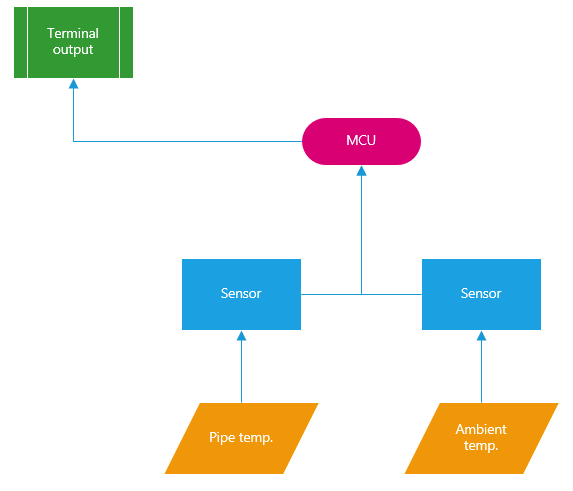
\includegraphics[width=0.5\textwidth]{figures/Phase1.PNG}
\end{figure}








